\documentclass[11pt]{beamer}
\usetheme{Boadilla}
\usepackage[utf8]{inputenc}
\usepackage{amsmath}
\usepackage{amsfonts}
\usepackage{amssymb}
\author{Thee Vanichangkul}
\title{Python und IoT}
%\setbeamercovered{transparent} 
%\setbeamertemplate{navigation symbols}{} 
%\logo{} 
%\institute{} 
%\date{} 
\subject{} 
\begin{document}

\begin{frame}
\titlepage
\end{frame}

\begin{frame}
	\frametitle{Was ist IoT?}
	\begin{quotation}
		"Das Internet der Dinge ist die technische Vision, Objekte beliebiger Art in ein universales digitales Netz zu integrieren. -wissenschaftliche Dienst des Deutschen Bundestages
	\end{quotation}
\end{frame}

\begin{frame}
	\frametitle{Anwendungsfall: Homeautomation}
	\begin{center}
		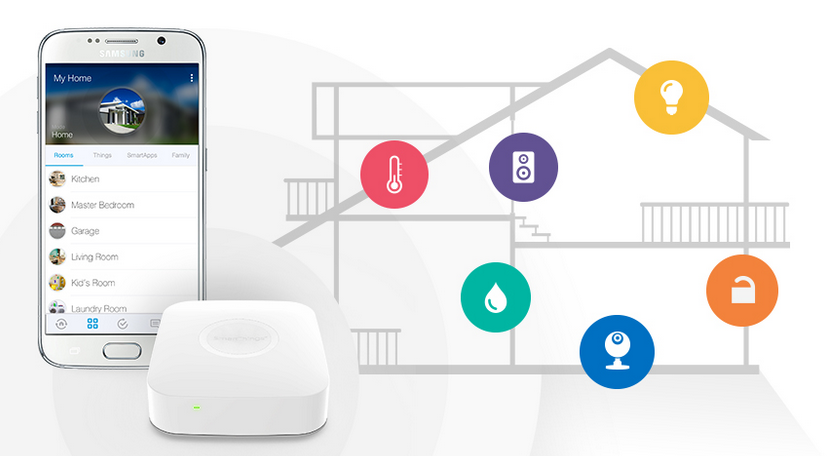
\includegraphics[width=0.8\textwidth]{Samsung_Hub.png}
	\end{center}
\end{frame}

\begin{frame}
	\frametitle{Die Dinge brauchen ein Protokoll!}
	\begin{center}
		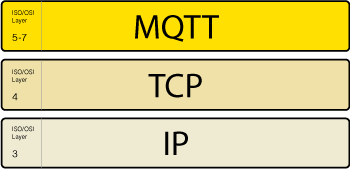
\includegraphics[width=0.7\textwidth]{mqtt-tcp-ip-stack.png}
	\end{center}
\end{frame}

\begin{frame}
	\frametitle{Was ist MQTT?}
	
\includegraphics[width=0.2\textwidth]{mqtt.png}
	\begin{itemize}
		\item MQTT (Message Queue Telemetry Transport)
		\item ein Messaging Protokoll für M2M Kommunikation 
		\item wurde von Mitarbeiter der IBM und Arcom im jahr 1999 entwickelt.
		\item Seit 2010 ist die Protokollspezifikation in Version 3.1 lizenzfrei verfügbar
	\end{itemize}
\end{frame}

\begin{frame}
	\frametitle{Warum MQTT?} 
	\begin{itemize}
		\item schlank
		\item einfach
		\item geeignet für ressourcenbeschränkte Geräte
	\end{itemize}
\end{frame}

\begin{frame}
	\frametitle{Wie funktioniert MQTT?} 
	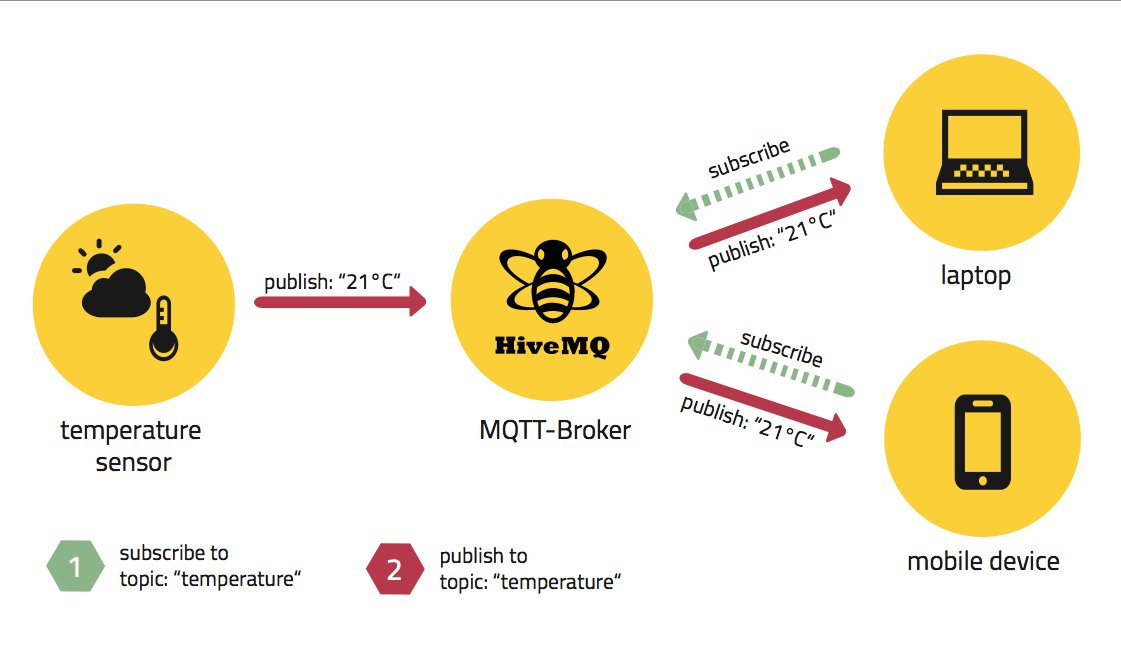
\includegraphics[width=1\textwidth]{hivemq.png}
\end{frame}

\begin{frame}
	\frametitle{MQTT Topic}
	\begin{center}
		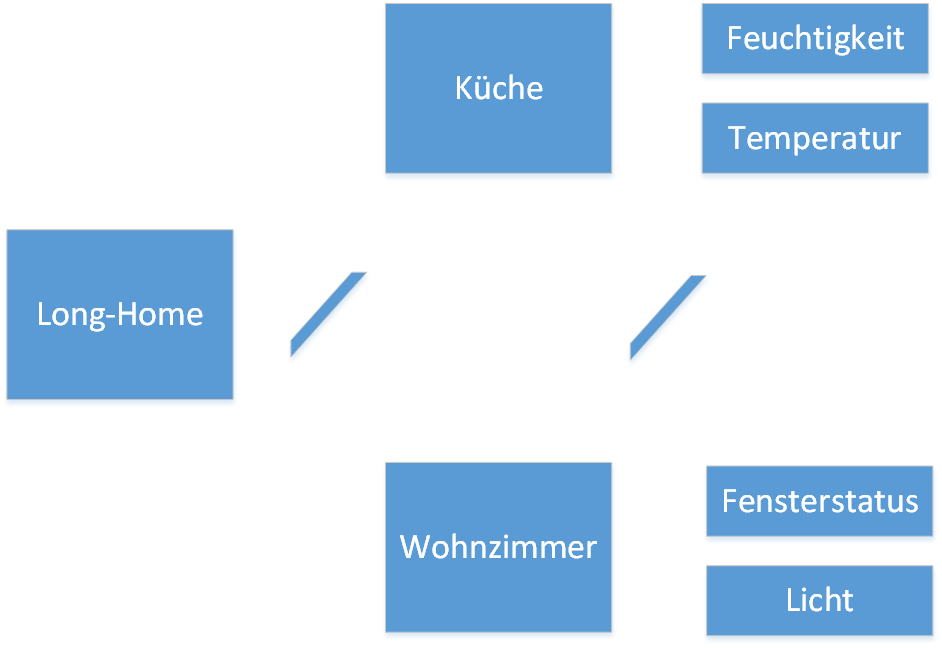
\includegraphics[width=0.7\textwidth]{mqtttopic.png}
	\end{center}
\end{frame}

\begin{frame}
	\frametitle{Mehr über Topic} 
	\begin{exampleblock}
		{Nur die Temperatur aus Longs Küche} \ Subscriber: Long-Home/Küche/Temperatur
	\end{exampleblock}
	\begin{exampleblock}
		{Alles aus Longs Wohnzimmer} \ Subscriber: Long-Home/Wohnzimmer/\#
	\end{exampleblock}
	\begin{exampleblock}
		{Alles aus Long-Home} \ Subscriber: Long-Home/\#
	\end{exampleblock}
	\begin{exampleblock}
		{Temperatursensor wert publishen} \ Publisher: Long-Home/Küche/Temperatur + "wert"
	\end{exampleblock}
\end{frame}

\begin{frame}
	\frametitle{Quality of Service (QoS)} 
	\begin{itemize}
		\item QoS 0: "nur ein mal" (best effort) “fire and forget”
		\item QoS 1: "Mindesten ein mal"
		\item QoS 2: "Wirklich nur ein mal"
	\end{itemize}
\end{frame}

\begin{frame}
	\frametitle{Sicherheit}
	\begin{itemize}
		\item Absicherung über Benutzername und Passwort.
		\item Transportebene mit SSL bzw. TLS verschlüsseln
		\item Authentifizierung mit Client Zertifikate oder über Access Control Lists z.B. durch die Überprüfung der IP einschränken.
	\end{itemize}
\end{frame}

\begin{frame}
	\frametitle{MQTT mit Python: Eclipse Paho} 
	\begin{itemize}
		\item Eclipse Paho ist ein Projekt unter dem Schirm der Eclipse Foundation
		\item Clientimplimentierungen für verschiedene Programmiersprachen verfügbar
		\item Existiert seit 2012
		\item Beitet auch ein Test-Server 
	\end{itemize}
\end{frame}

\begin{frame}
	\frametitle{Wie installiere ich MQTT?} 
		\begin{exampleblock}
		{Installation} \$ pip install paho-mqtt
	\end{exampleblock}
\end{frame}

\begin{frame}
	\frametitle{Code} 
\end{frame}

\begin{frame}
	\frametitle{Fragen?}
	\begin{center}
		Vielen Dank für Ihre Aufmerksamkeit!
	\end{center}
\end{frame}


\end{document}